\chapter{Blockchain Oracles} \label{chap:sota}

\section*{}
%Neste capítulo é descrito o estado da arte e são apresentados trabalhos relacionados para mostrar o que existe no mesmo domínio e quais os problemas em aberto. Deve deixar claro que existe uma oportunidade de desenvolvimento que cobre alguma falha concreta .

%O capítulo deve também efetuar uma revisão tecnológica às principais ferramentas utilizáveis no âmbito do projeto, justificando futuras escolhas.


The topic of blockchain oracles is still unexplored territory mostly investigated by start-up companies and individuals thriving to solve a new problem. Therefore, research related to oracles is scarcely found on peer-reviewed publications but, nonetheless, is invaluable in such an early phase of the technology. Consequently, the state of the art cannot be complete without reviewing the work developed by the academia and also by start-ups, enterprises, governments and individuals.

\section{Literature Review}

To get an overview of academic research a systematic literature review was performed. It's main components and finding are described in this section.

A literature review allows scholars not to step on each other's shoes but to climb on each other's shoulders, meaning, not duplicated existing research, find research gaps and strive to discover something new. To conduct a non-biased, methodical and reproducible review we identify its methodology, what are the data sources and what is the selection selection criteria (see \ref{search-process}).

The goal of this literature review is to get a sense of the corpus of existing works on the topic of blockchain oracles, and the directions and extent to which previous research has rendered significant results.

\subsection{Research Questions}
First of all and to guide the focus of the research, the following research questions were defined:
\begin{itemize}
  \item \textbf{RQ1:\label{RQ1} What kind of blockchain oracles have been proposed?}\newline We seek to analyse the scope of existing blockchain oracles. The methodologies and technologies used, so as to understand how the oracle problem is tackled.
  \item \textbf{RQ2:\label{RQ2} What are the research trends on blockchain oracles?}\newline The goal of this question is to identify the main directions of research. Analysing past solutions that never made it into production and solutions currently adopted.
\end{itemize}


\subsection{Search Process}\label{search-process}
Figure \ref{fig:/figures/SLR_stages}, depicts the predefined review strategy that was used. These steps are inspired on the guidelines for performing a systematic review by Kitchenham et al., 2007 \cite{Kitchenham2007}.

\begin{figure*}[h]
  \begin{center}
    \leavevmode
    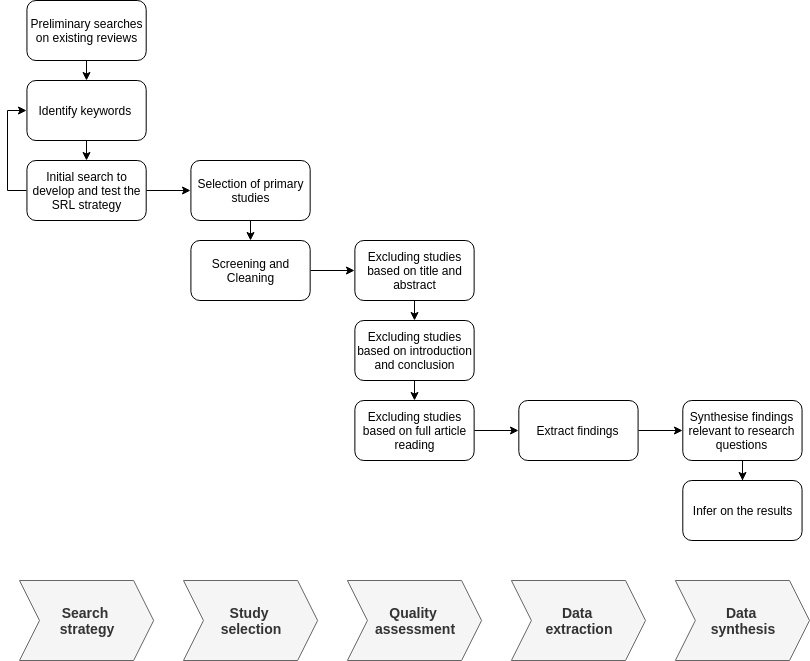
\includegraphics[width=\textwidth]{SLR_stages.png}
    \caption{Review strategy.}
    \label{fig:/figures/SLR_stages}
  \end{center}
\end{figure*}

The first step, \textbf{Search Strategy and Data-sources}, comprises a preliminary search on several databases trying to optimize the query that best fits the research questions. After identifying the set of keywords that best describe the problem a full query is built and tested.

Once a satisfactory query is achieved, we proceed to the next step, \textbf{Study selection}, here we aggregate the studies from all databases and in the \textit{Screening and cleaning} phase we remove papers written in other languages or duplicated.

Next, in the \textbf{Quality assessment} step we iteratively exclude papers that do not help us answer to any of the research questions. Initially analysing only the title followed by the abstract and so on until a full read of the article seems worth it to take conclusions and respond to que research queries.

This leads to the \textbf{Data extraction} step, in which we take and summarize the findings after reading each paper.

These findings are used in the \textbf{Data synthesis} step, we can summarize all the findings, infer some conclusions and answer the research questions.

\subsection{Search Strategy and Data-sources}

Having defined the strategy for the systematic review and after testing some keywords on multiple databases, the author selected the following four electronic databases to query for relevant information:

\begin{itemize}
  \item ACM Digital Library
  \item IEEE Xplore
  \item Scopus
  \item Google Scholar
\end{itemize}


The defined search query was the following:

\texttt{
  (("blockchain" OR "block chain" OR "block-chain")
  AND
  ("oracles" OR "oracle" OR "middle-ware" OR "middleware" OR "middle ware" OR "datafeed" OR "data feed" OR "data-feed"))
}

This search query was used to comprise all the possible ways of referring to blockchain and oracles. Some scholars have investigated the oracle issue by simply calling them a middleware or data-feed since oracles can either be used as an intermediary that relays data or as the source of the data.

The search was performed on the 5th of February 2019 and revealed the results presented in Table \ref{search-results-table}.


\begin{table*}[h]
  \begin{minipage}[c]{\textwidth}
    \centering
    \resizebox{0.7\textwidth}{!}{%
      \begin{tabular}{llr}
        \hline
        \textbf{Database}   & \textbf{Filters}                & \textbf{Results} \\ \hline
        ACM Digital Library & Title, abstract and keywords    & 34               \\
        IEEE Xplore         & Title, abstract and index terms & 24               \\
        Scopus              & Title, abstract and keywords    & 57               \\
        Google Scholar      & Title                           & 8                \\ \hline
        \textbf{Total}      & \textbf{}                       & \textbf{123}     \\ \hline
      \end{tabular}
    }
    \caption{Number of results and applied filters per database}
    \label{search-results-table}
  \end{minipage}
\end{table*}

Since the concept of smart contracts on the blockchain was only introduced in 2015, with the introduction of the Ethereum blockchain~\cite{GavinWood2014}, only results after 2015 were considered, also, all duplicated papers were removed. Analysing the initial search results per year, Figure \ref{search-results-per-year}, we can infer the growing popularity of oracle-related academic research. The year 2019 only comprises work published in the month of January since the search was performed at the beginning of February.

\begin{figure}[H]
  \centering
  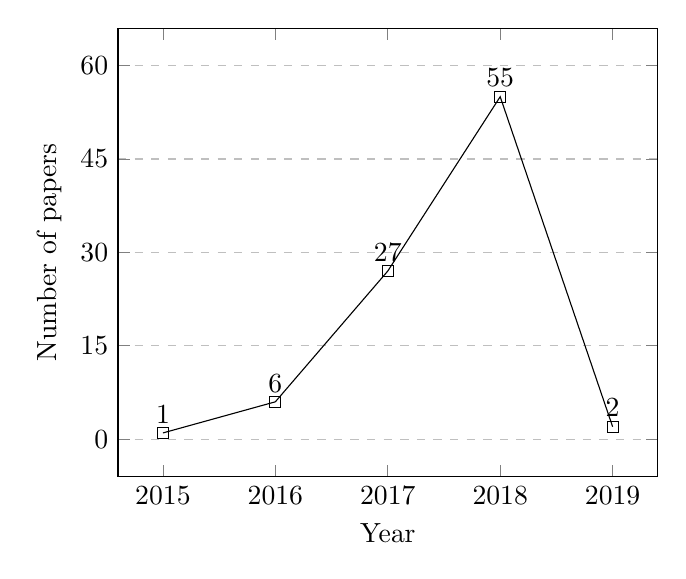
\begin{tikzpicture}
    \begin{axis}[
        xlabel={Year},
        ylabel={Number of papers},
        xtick=data,
        x tick label style={
            /pgf/number format/1000 sep=},
        xmin=2015, xmax=2019,
        ymin=0, ymax=60,
        ytick={0,15,30,45,60,75},
        ymajorgrids=true,
        grid style=dashed,
        enlargelimits=0.10,
      ]

      \addplot[
        mark=square, nodes near coords
      ]
      coordinates {
          (2015,1)(2016,6)(2017,27)(2018,55)(2019,2)
        };

    \end{axis}
  \end{tikzpicture}
  \caption{Resulting papers from search distributed per year}
  \label{search-results-per-year}
\end{figure}


\subsection{Study Selection and Quality Assessment}

The process of exclusion is depicted in Figure \ref{fig:/figures/paper-screening} and all the information regarding the papers and in which phase they were excluded is transparently presented in \ref{ap1:slr}.

The study selection process initially started with a pool of 123 papers from the previously stated online databases. As described on Figure \ref{fig:/figures/SLR_stages}, the selection and quality assessment compromised four stages:
\begin{itemize}
  \item Stage 1: Screening and cleaning duplicated articles or articles that were not in English.
  \item Stage 2: Exclusion by carefully reading the title but most importantly the abstract. After this stage, only 13 of the 91 non-duplicated papers were either describing specific trustable oracle implementations or mentioning the use of oracles.
  \item Stage 3: Analysing the introduction and conclusions in order to remove papers which do not describe an implementation of a trustable oracle or a protocol to overcome the trust in oracles.
  \item Stage 4: Full article reading to assess if the final bucket of articles answers the research questions.
\end{itemize}

\begin{figure}[H]
  \begin{center}
    \leavevmode
    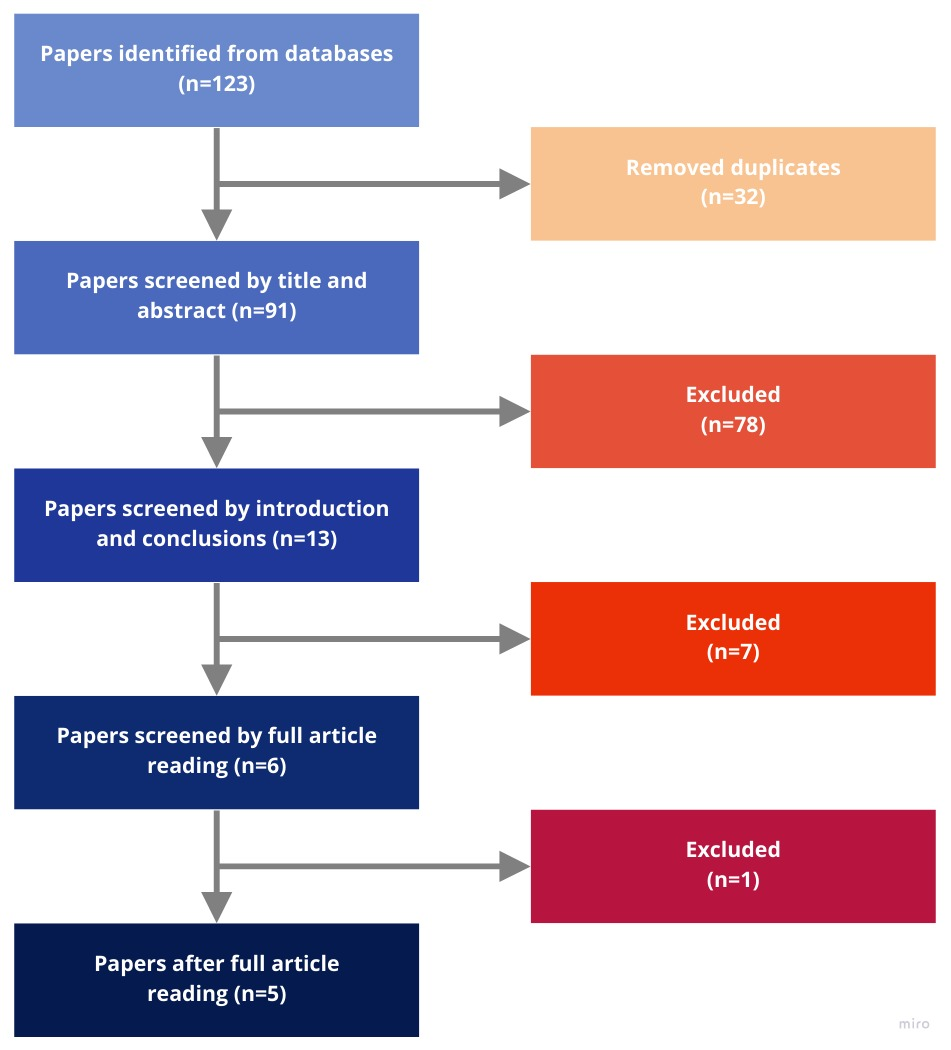
\includegraphics[width=0.7\textwidth]{figures/paper-screening.jpg}
    \caption{Screening stages.}
    \label{fig:/figures/paper-screening}
  \end{center}
\end{figure}

\subsection{Data extraction and Data Synthesis}\label{data-synthesis}

This process resulted in finding three articles and two theses that approach varying problems in implementing and guaranteeing trust in oracles. In these publications the author found the description of eight different implementations or approaches to blockchain oracles, which are analysed in the following paragraphs.

Town Crier (TC) \cite{Zhang2016a}, leverages trusted hardware, specifically Intel SGX\footnote{Intel Corporation. Intel® Software Guard Extensions SDK. https://software.intel.com/en-us/sgx-sdk, 2019}, to scrape HTTPS-enabled websites and serve source-authenticated data to smart contracts. The architecture of TC is depicted on Figure~\ref{fig:/figures/town-crier}~\footnote{Image taken from: https://town-crier.readthedocs.io/en/latest/how\_tc\_works.html}. It involves a TC contract on the blockchain that receives requests from a client contract and communicates those request to a TC server which runs a SGX-protected process to retrieve an answer from a data source through an HTTPS connection. Trusted Execution Environments (TEE) prevent even the operating system of the server from peeking into the enclave or modifying its behaviour, while use of the TLS (Transport Layer Security) protocol prevents tampering or eavesdropping on communications on the network.

\begin{figure}[H]
  \begin{center}
    \leavevmode
    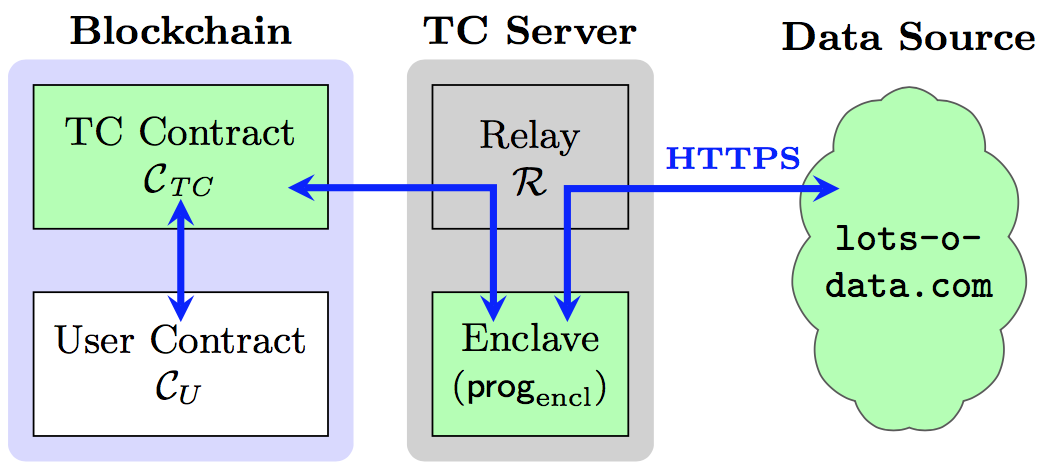
\includegraphics[width=0.45\textwidth]{figures/town-crier.png}
    \caption{Town crier high-level architecture. Figure taken from the Town Crier paper.}
    \label{fig:/figures/town-crier}
  \end{center}
\end{figure}


Astraea, proposed by \citet{Adler2018}, describes a decentralized oracle network, which is depicted on Figure~\ref{fig:/figures/astraea}~\cite{Adler2018a}, with submitters, voters and certifiers, in which voters play a low-risk game and certifiers a high-risk game with associated resources. Using a monetary incentive structure as a means to keep the players honest.

\begin{figure}[H]
  \begin{center}
    \leavevmode
    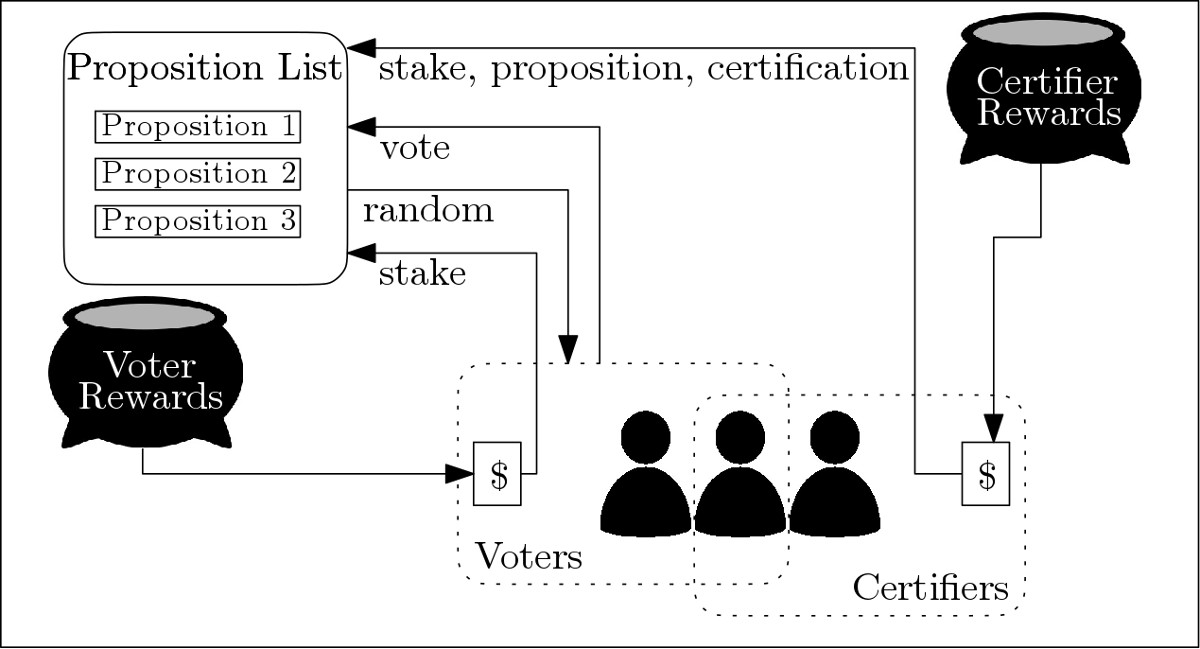
\includegraphics[width=0.7\textwidth]{figures/astraea.jpg}
    \caption{High-level overview of Astraea's architecture.}
    \label{fig:/figures/astraea}
  \end{center}
\end{figure}


Gilroy Gordon \cite{Gordon2017} proposes a protocol for oracle sensor data authenticity and integrity to IoT devices network with low computational resources. Using sets of public and private keys to authenticate that the oracle sensor data actually was originated by that oracle even if the information needs to pass by several oracles before being consumed by the application.

Francisco Monroy \cite{MontotoMonroy2018} defines a gambling protocol based on incentives and assuming that every entity involved has the objective to maximize their profit. The protocol overcomes the trust in a single Oracle by polling a network of 7 oracles from a large network of available oracles, they will then stake their money on a specific bet and only receive their investment back if the majority of the oracles vote in the same winner. Creating, therefore, incentives for Oracle good behaviour.


J. Eberhardt \cite{Eberhardt2018} does not propose a specific method but analyses existing solutions and defines a systematic classification for existing trustable off-chain computation oracles. The authors identify the following off-chain computation oracles approaches:


\begin{itemize}
  \item \textit{Verifiable off-chain Computation}, a technique where a prover executes a computation and then publishes the result including a cryptographic proof attesting the computation’s correctness to the blockchain. An on-chain verifier then verifies the proof and persists the result in case of success. Identified existing solutions are zkSNARKs~\cite{Ben-SassonTechnionAlessandroChiesa2019}, Bulletproofs~\cite{Bunz2018} and zkSTARKs~\cite{Ben-Sasson2018}. zkSNARKs require a setup phase which is more expensive than naive execution. After the setup, however, proof size and verification complexity are extremely small and independent of circuit complexity. This amortization makes zkSNARKs especially efficient for computations executed repeatedly, which is usually the case for off-chain state transitions. While zkSTARKs and Bulletproofs require no setup, proof size and verification complexity grows with circuit complexity, which limits applicability.
  \item \textit{Secure Multiparty Computation}, SMPCs, enable a set of nodes to compute functions on secret data in a way that none of the nodes ever has access to the data in its entirety. Identifies Enigma~\cite{Tam2018}, which proposes a privacy-preserving decentralized computation platform based on multiple parties where a blockchain stores a publicly verifiable audit trail. However, current SMPC protocols add too much overhead for them to be practical. Hence, Enigma now relies on Trusted Execution Environments.
  \item \textit{Enclave-based Computation}, EbC, relying on Trusted Execution Environments (TEE) to execute computations off-chain. Identified existing solutions are Enigma and Ekiden \cite{Cheng2018} which present two different implementations of EbCs. In Enigma, programs can either be executed on-chain or in enclaves that are distributed across a separate off-chain network. An Enigma-specific scripting language allows developers to mark objects as private and hence, enforce off-chain computation. In contrast to Enigma, Ekiden does not allow on-chain computation but instead, the blockchain is solely used as persistent state storage.
  \item \textit{Incentive-driven Off-chain Computation}, IOC, relies on incentive mechanisms applied to motivate off-chain computation and guarantee computational correctness. IOCs inherit two critical design issues: (1) keep verifiers motivated to validate solutions and (2) reduce computational effort for the on-chain judge. The paper identifies TrueBit~\cite{Teutsch2017}, as the first IOC implementation, proposing solutions for both challenges. As verifiers would stop validating if solvers only published correct solutions, TrueBit enforces solvers to provide erroneous solutions from time to time and offers a reward to the verifiers for finding them.
\end{itemize}




\section{Commercial Products and Projects}\label{sec:4}

This search, unlike the systematic one explained before, cannot be described in a systematic way, since the source of the information is scattered throughout whitepapers and documentation webpages of startups, which cannot be guaranteed to be searchable and assessable in a systematic way.

To search for existing commercial products and projects, Google, a search engine and Medium, a platform for blog posting used widely by developers and the start-up community, were used as a means to find new projects or solutions for the oracle trust problem. Using these two tools a lot of projects were found trying to solve the oracle trust problem and are solely documented on white-papers or on the companies' website documentation page. This kind of literature cannot be found in peer-reviewed databases, but can nonetheless provide invaluable information and is therefore worth being analysed.

The results of this search revealed a wide range of projects and protocols with varying degrees of decentralization or authenticity. A short explanation of each will be detailed here:

\begin{itemize}
  \item Oraclize.it \cite{Oraclize.it2018}, provides Authenticity Proofs for the data it fetches guaranteeing that the original data-source is genuine and untampered and can even make use of several data sources in order the gather trustable data, but its centralized model does not guarantee an always available service.
  \item ChainLink\cite{Ellis2017}, describes a decentralized network of oracles that can query multiple sources in order to avoid dependency of a sole oracle, which can be prone to failure and also to gather knowledge from multiple sources to obtain a more reliable result. ChainLink is also considering implementing, in the future, authenticity proofs and make use of trusted hardware, as of now it requires users to trust in the ChainLink nodes to behave correctly.
  \item SchellingCoin~\cite{VitalikButerin2014} protocol incentivizes a decentralized network of oracles to perform computation by rewarding participants who submit results that are closest to the median of all submitted results in a commit-reveal process.
  \item TrueBit~\cite{Teutsch2017}, introduces a system of solvers and verifiers. Solvers are compensated for performing computation and verifiers are compensated for detecting errors in solutions submitted by solvers.
\end{itemize}


\section{Summary}

A detailed explanation of the findings from the systematic literature search is already detailed in Section~\ref{data-synthesis} and the industry solutions in Section~\ref{sec:4}. This section analyses the combined work from both the academia and industry.

Table \ref{oracle-summary}, summarises the existing projects that were found and answers the first research question (Section \ref{RQ1}) highlighting three main types of oracles.

\begin{table}[]
  \centering
  \resizebox{\textwidth}{!}{%
  \begin{tabular}{lccl}
    \hline
    Name                      & Type                       & Distributed Network & Achieves trust through                         \\ \hline
    Town Crier                & Hardware-based             & No                  & Trusted hardware signed attestations           \\
    Astraea                   & Consensus-based            & Yes                 & Network with submitters,  voters and certifier \\
    \citet{Gordon2017}        & Software-based             & Yes                 & Sets of public and private keys                \\
    \citet{MontotoMonroy2018} & Consensus-based            & Yes                 & Gambling protocol based on incentives          \\
    TrueBit                   & Consensus-based            & Yes                 & System of solvers and verifiers                \\
    Oraclize.it               & Software-based             & No                  & TLSNotary, Android Proof                       \\
    ChainLink                 & \begin{tabular}[c]{@{}c@{}}Consensus-based /\\ Software-based\end{tabular} & Yes                 & Query multiple sources                         \\
    SchellingCoin             & Consensus-based            & Yes                 & Incentive based                                \\ \hline
  \end{tabular}%
  }
  \caption{Summary of oracle projects/research.}
  \label{oracle-summary}
\end{table}

The first is \textbf{software-based oracles}, which try to prove their honest behaviour through the use of software-based authenticity proofs. These, mostly take advantage of some features of TLS to prove that the data they are relaying is the actually provided data.

The second type is \textbf{hardware-based oracles}. These leverage specific hardware to provide a TEE, to securely separate the environment running the oracle code from the operating system and other applications to achieve higher guarantees on untampered code execution. They may even provide authenticity proofs regarding that the query actually came from a legit TEE.

Lastly, \textbf{consensus-based oracles}, which require a network of peers working together to achieve higher redundancy, having several peers querying the data and even in some cases peers performing the role of the verifier. This last approach largely depends on the existence of such a network and requires the use of monetary incentives to keep the networking running.

The most promising solutions are Town Crier, ChainLink and Oraclize.it .  Town Crier hardware-based solution, more specifically Intel SGX, adds strong guarantees that the computation performed can be trusted due to its isolution from the remaining environment. To this reason, ChainLink is adopting Town Crier\footnote{ChainLink's annoucement regarding the use of Town Crier: https://blog.chain.link/town-crier-and-chainlink/} to add increasing reliability to their distributed solution. The ChainLink distributed oracle network and their partnerships with huge players such as SWIFT~\footnote{SWIFT is a global provider
  of secure financial messaging services, more info: https://www.swift.com/} make it a promising solution, although a private and fee-based one.

Oraclize.it, is an industry leading service because of their use and research of authenticity proofs. They have also integrations with the most widely used blockchains implementations, such as, Ethereum, EOS~\cite{Block.one2018}, Hyperledger Fabric~\cite{Androulaki}, Rootstock~\footnote{More information on Rootstock can be found here: https://www.rsk.co/} and Corda~\cite{Brown2016}. Their authenticity proofs are both software-based and hardware-based, with the use of TLSNotary~\cite{TLSnotary}, Android Proof~\footnote{More information on the Android Proof can be found here: https://provable.xyz/papers/android\_proof-rev2.pdf} and Ledger Proof~\footnote{More information on the Ledger Proof can be found here: https://docs.provable.xyz/\#security-deepdive-authenticity-proofstypes-ledger-proof}.

In conclusion, the industry presents ready to use solutions for a fee where as the academia mostly investigates the use of consensus-based solutions which adopt an incentives based network. The latter has the problem of requiring such a network of peers to existing in order to be trusted where as the former can be used right away.

\section{Conclusions}

The author surveys 123 papers and fully analyses 5. One resulting in an hardware-based oracle solutions, two consensus-based oracle proposals, one software-based solution for an IoT devices network data authentication and the last one proposing a classification system of existing off-chain computation oracles. The industry presents us four projects, in which two of them are widely in use, namely Oraclize.it and ChainLink, and other two consensus-based solutions. The industry seems to be investing the most on oracle research, as the two previous mentioned companies are developing a wide range of authenticity proofs and leverage hardware solutions to increase their oracles trustability as details on the previous section. As well as partnering with major banks and institutions to allow their solutions to power new solutions for smart contracts.

Two main conclusions arise from both academic and non-academic research, and answer the second research question \ref{RQ2}.

First of all, there is a clear lack of academic research on the topic of creating trustable oracles. This is mostly likely due to the specificity of the problem and that blockchain related technology is usually paved by start ups and enthusiasts and not yet addressed in universities curricular plans.

Secondly, even though the main research on trustable oracles is being pursued by startups or sole developers all the existing projects seem to be blockchain specific or in very early phases and not yet ready to be generally adopted.
